\documentclass{article}
\usepackage{amsmath}
\usepackage{amsfonts}
\usepackage[english]{babel}
\usepackage[utf8]{inputenc}
\usepackage{amsthm}
\usepackage{graphicx}
\usepackage{array}
\usepackage{tabularx}

\newcommand{\norm}[1]{\left\lVert#1\right\rVert}
\newtheorem{theorem}{Theorem}
\newtheorem{prop}{Proposition}

\begin{document}

\title{Parallel Processing Homework 1}
\author{Toby Harvey}
\maketitle


In this homework I implemented 2 different algorithm for calculating pi. I found that the fastest implementation of the numerical quadrature method of calculating pi used openmp's for loop where each ``bar'' calculated by a thread is summed using a reduction. This is significantly faster than protecting the memory location of the sum using openmp's atomic. I would think that this is because atomic just causes some serialization when protecting memory whereas reduction implements an actual parallel reduction algorithm (maybe something with pipe-lining) so it does much less serializing. Interestingly, the difference between using atomic and a reduction in the Monte-Carlo algorithm is negligible. I am having a hard time coming up with a hypothesis as to why that is. Parallelizing the Monte-Carlo simulation with either method does not give any speed up, and I believe this is because the overhead of initializing threads cancels out the time saved doing any parallel computations because each thread only does an addition and write (see line 269 of pi.c). Although, this gives no insight into why the reduction and atomic perform the same for the Monte-Carlo implementation. Lastly on the whole the Monte-Carlo calculation is probably slower because the random number generation for each iteration is significantly more expensive than the calculations for each quadrature point.

After determining that the reduction quadrature version performed the best, I tested it with a varying number of threads from 1 (serial) to 32. The performance was pretty much the same except for (obviously) 1 and 8 threads. I ran my code on a 6 core, 12 processor machine. Why 8 threads is particularly bad is unclear to me.

The convergence rate is significantly faster for quadrature than it is for the Monte-Carlo. The best explanation I can think of for this is that while the random number generator is uniformly distributed between -1 and 1 any given number of draws will be bias somewhere within the domain leading to a too low or too high number of counts inside the circle ultimately leading to slower convergence with number of samples. This begs the question why even do any random number generation? Why not just generate a grid of points and count which ones lie in the circle? It is possible that this technique would lead to faster convergence with grid refinement. I am also curious if finite precision leads to slower convergence, but I am unsure.


\begin{table}
  \caption {Convergence for Calculating Pi} \label{tab:title} 
  \small
\begin{flushleft}
\begin{tabular} {| c | c | c | c | c | c | c |}
  \hline
  $\log_{10} \# points$ & serial quad & reduct quad & atomic quad & serial monte & reduct monte & atomic monte \\
  \hline
  1 & 3.0370488289 & 3.0370488289 & 3.0370488289 & 3.2000000000 & 4.0000000000 & 4.0000000000 \\

  2 & 3.1382685111 & 3.1382685111 & 3.1382685111 & 2.8800000000 & 3.0000000000 & 3.4400000000 \\

  3 & 3.1414874770 & 3.1414874770 & 3.1414874770 & 3.0880000000 & 3.0720000000 & 3.1080000000 \\

  4 & 3.1415893274 & 3.1415893274 & 3.1415893274 & 3.1196000000 & 3.1500000000 & 3.1428000000 \\

  5 & 3.1415925484 & 3.1415925484 & 3.1415925484 & 3.1437600000 & 3.1499200000 & 3.1463200000 \\

  6 & 3.1415926503 & 3.1415926503 & 3.1415926503 & 3.1428720000 & 3.1413920000 & 3.1394240000 \\
  
  7 & 3.1415926535 & 3.1415926535 & 3.1415926535 & 3.1422560000 & 3.1413380000 & 3.1412680000 \\
\end{tabular}
\end{flushleft}
\end{table}


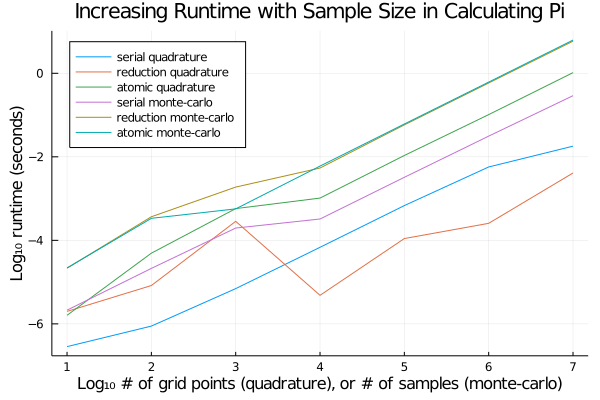
\includegraphics[scale=.45]{hw1_plot.png}

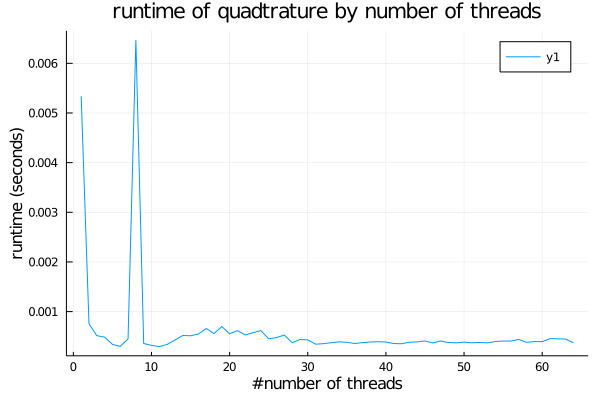
\includegraphics[scale=.45]{threads_runtime.png}

\end{document}
